\documentclass[pdf]{beamer}

\usetheme[richting=SE, logo=ENG]{HvA}

\usepackage[utf8]{inputenc}
\usepackage{hyperref}
\usepackage{complexity}
\usepackage{dirtytalk}
\usepackage{tabularx}
\usepackage[backend=biber,alldates=iso8601,autocite=footnote]{biblatex}

\bibliography{../quantum-simulation-research-paper}

\author{Steven Oud}
\title{{\LARGE Solving Hard Scientific Problems Using Quantum Computers}}
\subtitle{Progress Presentation}
\institute{Hogeschool van Amsterdam}
\date{\today}

\begin{document}
    \frame{\titlepage}
    
    \begin{frame}
    	\frametitle{Table of contents}
        \tableofcontents
    \end{frame}

    \section{Quantum Computation and Information}
    \begin{frame}
        \frametitle{Quantum Computation and Information}
        Quantum computers take advantage of quantum mechanical effects such as superposition and interference to solve certain problems faster than classical computers.
    \end{frame}

    \begin{frame}
        \frametitle{Quantum Computation and Information: Qubits}
        \begin{itemize}
            \item Unlike a classical bit, a qubit can be in superposition of 0 and 1.
            \item In a superposition, each state has an amplitude, which can be a negative or positive complex number.
            \item When we measure a qubit, it collapses to 0 or 1 randomly.
            \item The amount of amplitudes grow exponentially with the number of qubits: a $n$-qubit system requires $2^n$ amplitudes to describe the system.
        \end{itemize}
    \end{frame}

    \begin{frame}
        \frametitle{Quantum Computation and Information: Interference}
        \begin{figure}[ht]
            \begin{minipage}{.56\textwidth}
                \say{The goal in quantum computing is to choreograph a computation so that the amplitudes leading to wrong answers cancel each other out, while the amplitudes leading to right answers reinforce.}
                - \textcite{aaronson2011quantum}
            \end{minipage}
            \hfill
            \begin{minipage}{.4\textwidth}
                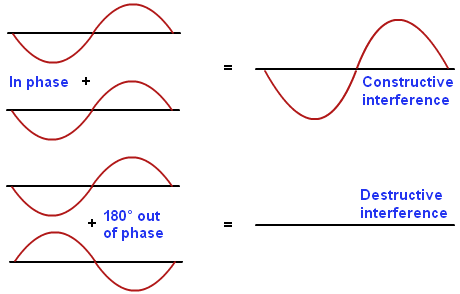
\includegraphics[width=1\linewidth]{../figures/interference.png}
            \end{minipage}
        \end{figure}
    \end{frame}

    \begin{frame}
        \frametitle{Quantum Computation and Information: Entanglement}
        Particles can interact and produce entangled states which show correlations in measurement outcomes.
        
        \vfill
        
        Example: Bob and Alice share two entangled electrons with opposite spins. When Bob measures his electron to be spin up, Alice's electron must be spin down and vice versa.
    \end{frame}

    \section{Quantum Computational Complexity}
    \begin{frame}
        \frametitle{Quantum Computational Complexity}
        \only<1>{
            \begin{itemize}
                \item We describe running time of an algorithm as a function of the size of the input~\cite{cormen2009introduction}.
                \item We usually concentrate on the worst-case running time of an algorithm.
                \item Problems in class $\P$: polynomial-time algorithms (``easy" problems) grow by some constant $k$ given input size $n$: $O(n^k)$.
                \item Porblems in class $\NP$: superpolynomial-time algorithms (``hard problems"), grow faster than $O(n^k)$, for example $O(2^n)$ or $O(n!)$.
            \end{itemize}
        }
        \only<2>{
            \begin{figure}[ht]
                \centering
                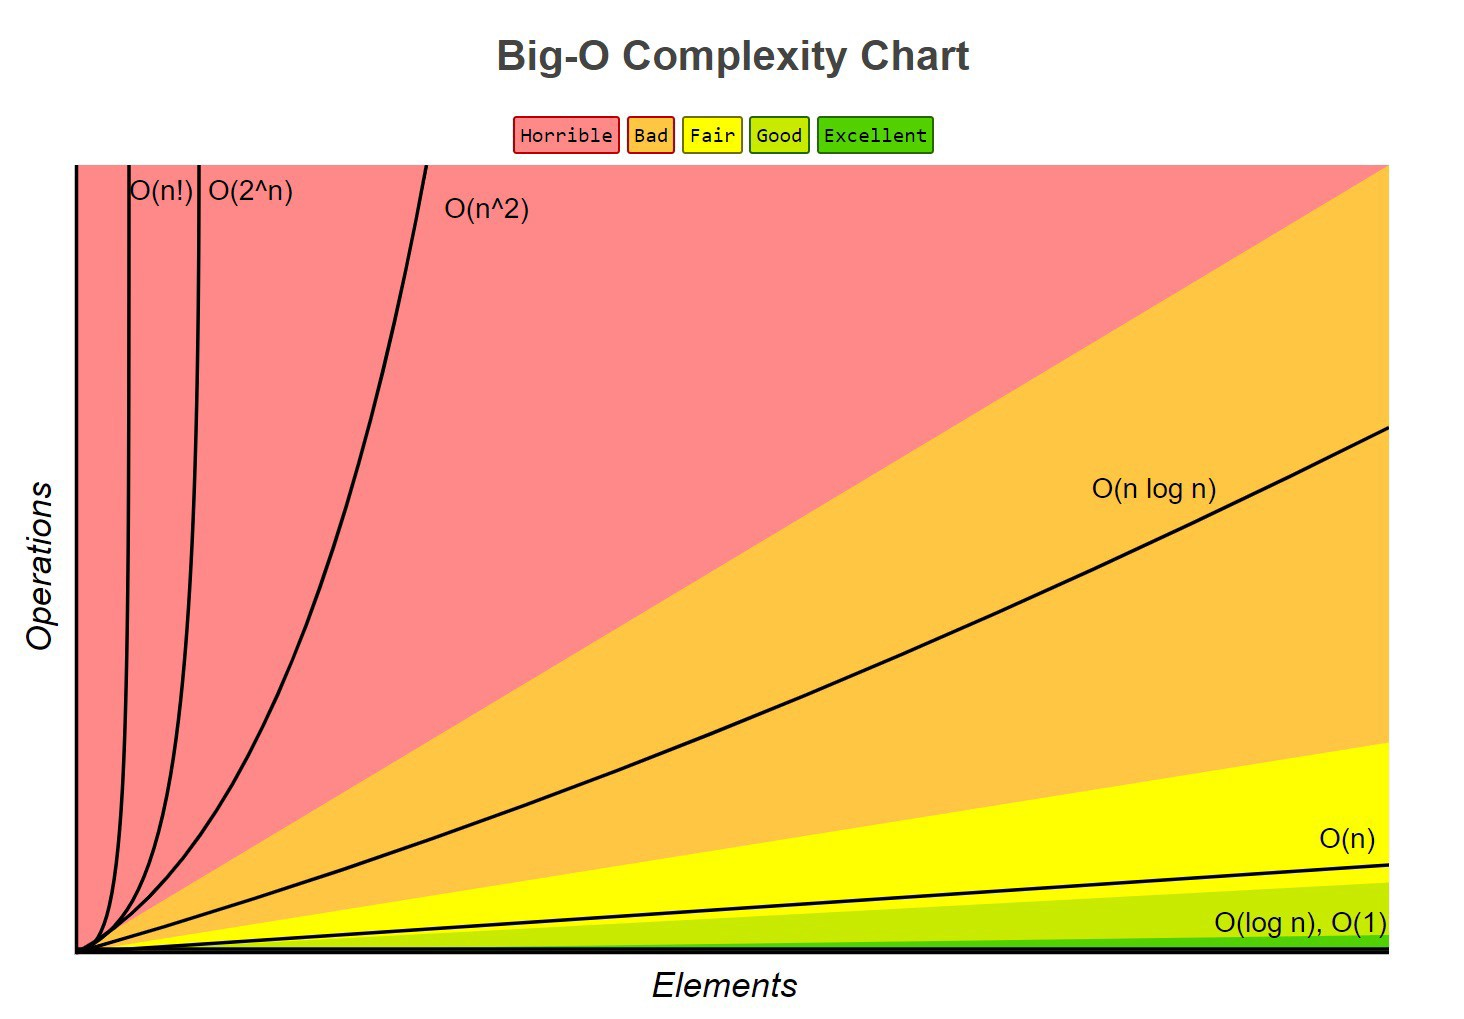
\includegraphics[width=.8\linewidth]{../figures/time_complexity.jpeg}
            \end{figure}
        }
        \only<3>{
            \begin{figure}[ht]
                \centering
                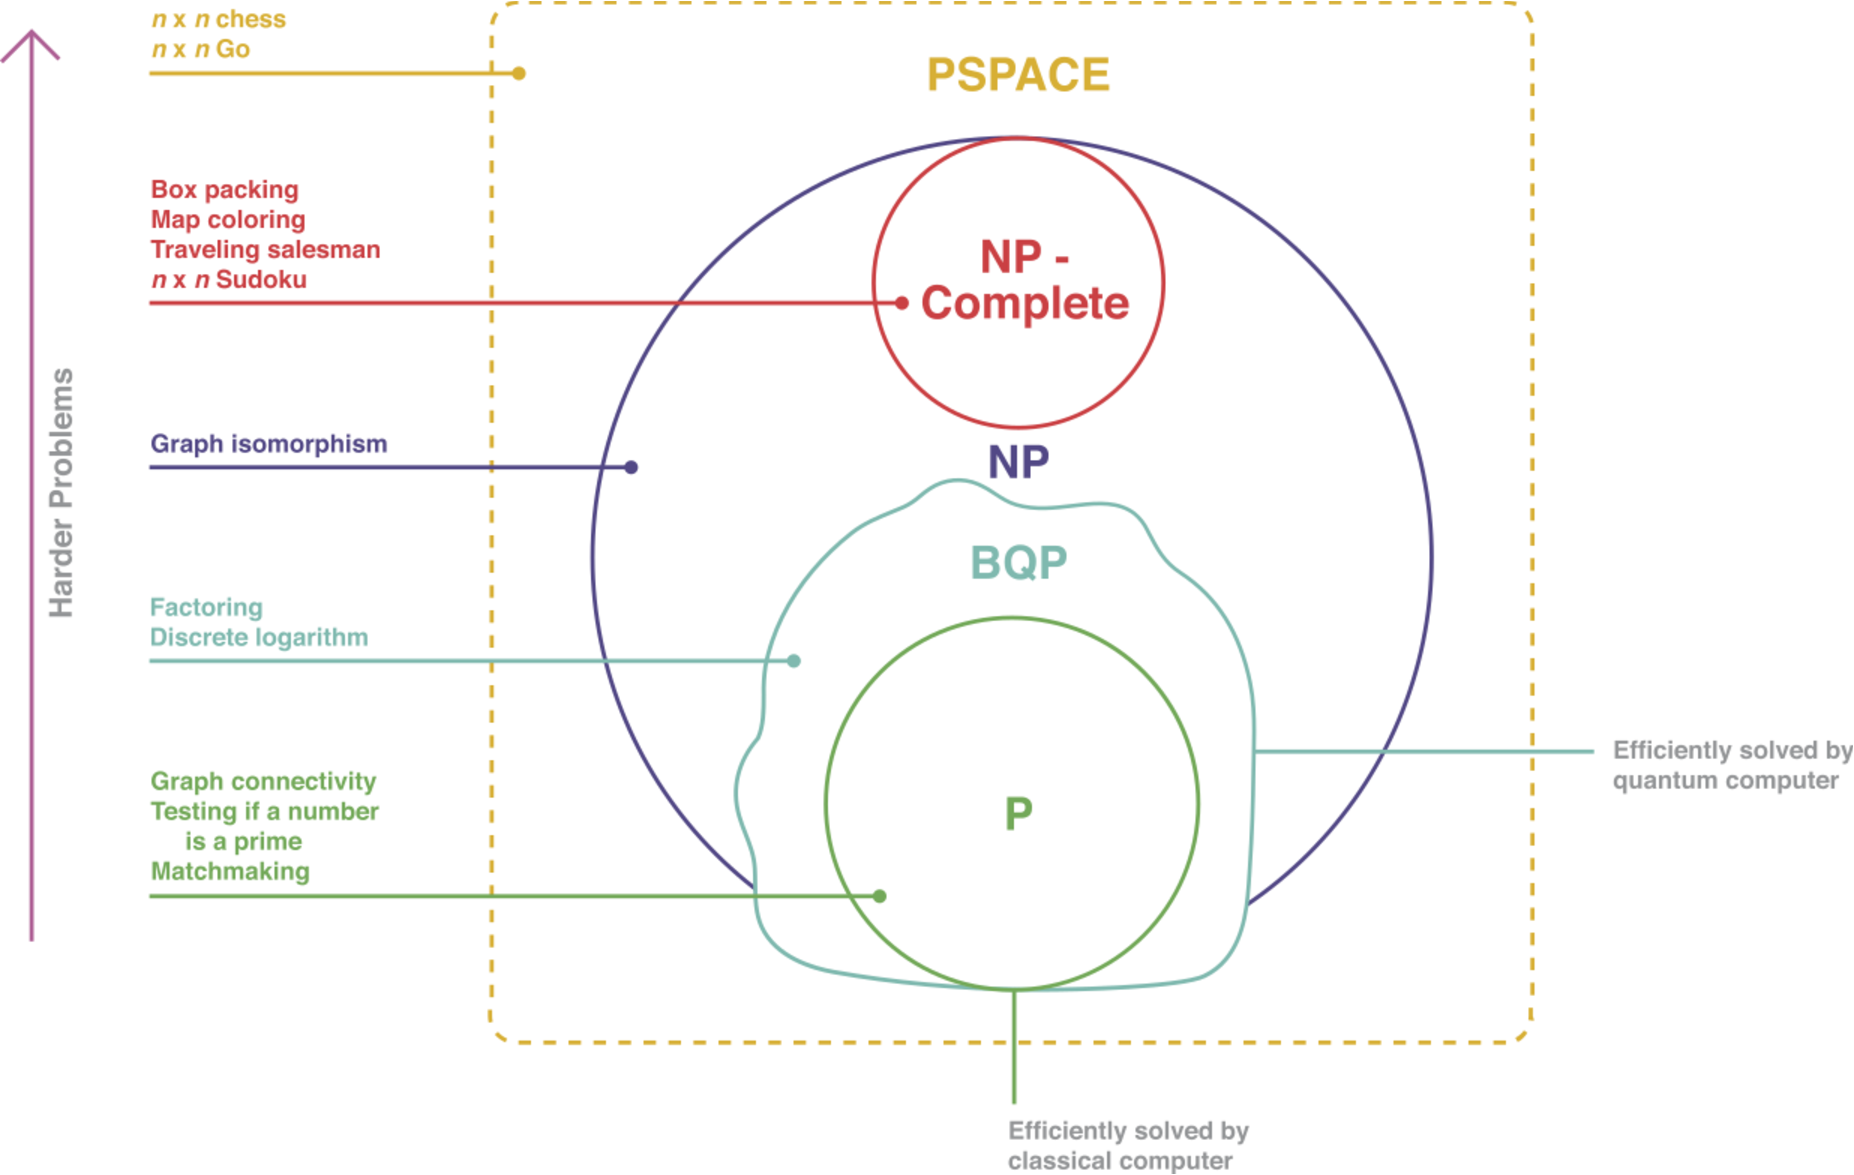
\includegraphics[width=.7\linewidth]{../figures/complexity_hierarchy.pdf}
                \caption{A diagram illustrating the hierarchy of several important complexity classes. Image by MIT OpenCourseWare.}
            \end{figure}
        }
        \only<4>{
            \begin{tabular}{c|c|c}
                \hline
                Algorithm & Quantum Speedup & Technique \\
                \hline
                Factoring & Superpolynomial & \cite{shor-factoring} \\
                Quantum Simulation & Superpolynomial &
                \cite{zalka1998efficient, lloyd1996universal, aspuru2005simulated} \\
                Searching & Polynomial & \cite{grover1996fast} \\
                Constraint Satisfaction & Polynomial & \cite{ambainis2005quantum} \\
                \hline
            \end{tabular}
        }
    \end{frame}

    \section{Quantum Computing for Scientific Problems: Quantum Chemistry}
    \begin{frame}
        \frametitle{Quantum Computing for Scientific Problems: Quantum Chemistry}
        Problem: find the minimum energy state of a molecule
        \only<1>{
        \begin{itemize}
            \item Since the founding of the field of quantum mechanics, we have been able to describe the state of a quantum-mechanical system by solving the Schr{\"o}dinger equation~\cite{griffiths2018introduction}.
            \item Applications in chemistry, biology, drug discovery, and materials science~\cite{mcardle2018quantum}.
        \end{itemize}
        }
        \only<2>{
        \begin{itemize}
            \item Unfit for classical computers: quantum system grows exponentially with the number of particles - requires an exponential amount of classical bits to represent the quantum system.
            \item Quantum state's amplitudes grows exponentially with the amount of qubits --- requires a linear amount of qubits to represent the quantum system.
        \end{itemize}
        }
        \only<3>{
            Quantum algorithms for finding the minimum energy state of a molecule:
            \begin{itemize}
                \item Quantum Phase Estimation (QPE) algorithm --- requires fault-tolerant quantum computer~\cite{nielsen-chuang}.
                \item Variational Quantum Eigensolver (VQE) --- candidate for near-term quantum devices using iterative classical optimization~\cite{vqe}.
            \end{itemize}
            
        }
    \end{frame}

    \section{Other Possible Scientific Applications for Quantum Computers}
    \begin{frame}
        \frametitle{Other Possible Scientific Applications for Quantum Computers}
        \begin{itemize}
            \item Machine learning
            \item Cryptography
            \item Biology (genome sequencing)
        \end{itemize}
    \end{frame}

    \begin{frame}[allowframebreaks]
        \setbeamertemplate{bibliography item}{\insertbiblabel}
        \vspace*{2em}
        \printbibliography
    \end{frame} 
\end{document}
